\documentclass[12pt]{article}
\usepackage[utf8]{inputenc}
\usepackage{graphicx}
\usepackage{float}
\usepackage{geometry}
\usepackage{url}
\usepackage{natbib}
\usepackage[hidelinks]{hyperref}
\geometry{a4paper, margin=1in}
\title{Software and Cultures Case Study \\ \large Virtualization in
    communication: post pandemic benefits and challenges}
\author{m5271506 Kiyohiro Murai}
\date{}

\begin{document}

\maketitle
\tableofcontents
\newpage

\section{Introduction}
In recent years, the virtualization of communications has changed the way we
communicate in business, education, and even personal life. This change was
particularly accelerated by the global crisis caused by the 2020 pandemic.
Lockdowns and the need for social distancing have led to digitalization in
areas such as virtual meetings, distance learning, and online entertainment.

During the pandemic, many companies transitioned to remote work. This
transition meant relying heavily on virtualization services for employees to
work from anywhere. Platforms such as
Zoom\footnote{https://www.zoom.com/en/products/virtual-meetings/}, Microsoft
Teams\footnote{https://www.microsoft.com/ja-jp/microsoft-teams/group-chat-software},
Slack\footnote{https://slack.com/intl/ja-jp}, and
Discord\footnote{https://discord.com/}, which will be discussed later, have
rapidly become popular
as everyday
communication tools\cite{zoom_status, teams_status, slack_status,
    discord_status}. These services not only virtualized meetings, but also
served as a venue for project management, document sharing, and even social
interaction.

The impact of the pandemic has significantly changed the way we look at remote
work and virtualized services. Many companies and organizations are rethinking
the need for physical offices and exploring a combination of flexible
workspaces and virtual meetings. This change has not only affected the
way we work, but also corporate culture, employee well-being, and productivity.

Post-pandemic, predictions about the future of remote work and virtualized
services vary. Some experts predict that many companies will move away from
fully remote work to a hybrid model. On the other hand, advances in
virtualization technology are expected to increase the number of companies that
will continue with a fully remote work style. These changes are likely
to drive further advances in virtualization technology and lead to the
emergence of new business models and work practices.

This case study provides an in-depth analysis of the impact virtualization has
had
on communication and work practices, and discusses the future of remote work
and virtualized services in a post-pandemic world. We also explore how the
expansion of remote work will impact individual lives and society as a whole.
We aim to identify the long-term benefits and challenges of this transformation
and provide direction for the future.

\section{What is virtualization}
In this case study, "virtualization" mainly refers to concepts in information
technology and communication. Virtualization technology refers to technology
that divides physical resources (e.g. servers, storage, network equipment,
etc.) into multiple virtual resources and uses them efficiently
\cite{virtualization_overview}.
Virtualization, especially in communications, is concerned with the realization
of communication that is independent of physical location. It enables
communication across geographic boundaries, allowing participants to attend
meetings and events from anywhere in the world. This greatly increases the
flexibility and accessibility of communication.

\newpage
\section{Virtualization services}
With the evolution of technology in recent years, virtualization services have
become an essential part of business and daily life. Many services were already
available before the pandemic. The pandemic has made these services even more
important. In this section, we will focus on major remote communication
services, video conferencing tools, comprehensive communication platforms,
virtual offices, and virtual environments using VR, AR, and MR, and provide an
overview and usage examples of them. These services are used not only for work
but also for a variety of purposes such as webinars, telemedicine/healthcare,
and document sharing. It can also be found used in cultural facilities and
entertainment fields. This has provided a way for people to enjoy culture and
entertainment across countries, cultures, and races, even under restrictions
during the pandemic.

\subsection{Video conferencing service}
Video conferencing service has become an important element of modern
communication. These services have overcome geographic constraints and enabled
people in remote locations to communicate face-to-face in real time. Video
conferencing is used for a wide variety of purposes, including business
meetings, webinars, education, healthcare, and personal interactions. This
technology is also important as it saves time and money, improves
accessibility, and provides a sustainable communication environment. Let's take
a look at some typical service examples.
\begin{table}[h]
    \begin{center}
        \begin{tabular}{|l|c|} \hline
            Service Name   & Release (Establishment) Year \\ \hline
            Zoom           & 2012                         \\
            Google Meet    & 2017                         \\
            Cisco WebEx    & 1995                         \\
            GoToMeeting    & 2004                         \\
            Adobe  Connect & 2005 (Acquisition)           \\
            BlueJeans      & 2009                         \\ \hline
        \end{tabular}
        \caption{Video conferencing service}
    \end{center}
\end{table}

Zoom is a popular service that was released in 2012 and offers a variety of
features such as video conferencing, webinars, live chat, and screen sharing.
Known for its easy operation and stable connection quality, it is widely used
not only for business but also for education and personal use.

Google Meet\footnote{https://workspace.google.com/intl/ja/products/meet/} is a
video conferencing service provided by Google, originally
provided as part of the G Suite web conferencing system (Hangouts Meet). The
service is designed for business users and educational institutions and
features a simple and easy-to-use interface.

Other services include
CiscoWebEx\footnote{https://www.webex.com/ja/video-conferencing.html} ,
GoToMeeting\footnote{https://www.goto.com/meeting}, Adobe
Connect\footnote{https://www.adobe.com/jp/products/adobeconnect.html}, and
BlueJeans\footnote{https://www.bluejeans.com/}.

\subsection{Voice call messaging tool}
Voice calling messaging tool is another important aspect of remote
communication. These tools enable instant communication between individuals and
groups and play an essential role in many aspects of business and personal
life.

\begin{table}[h]
    \begin{center}
        \begin{tabular}{|l|c|} \hline
            Service Name & Release (Establishment) Year \\ \hline
            Skype        & 2004                         \\
            WhatsApp     & 2009                         \\
            Viber        & 2010                         \\ \hline
        \end{tabular}
        \caption{Voice call messaging tool}
    \end{center}
\end{table}

Skype\footnote{https://www.skype.com/ja/} provides voice calling, video
calling, and instant messaging services for
both personal and business users. Another feature is low-cost international
calls.

WhatsApp\footnote{https://www.whatsapp.com/?lang=ja} is a globally popular app
that offers free messaging and voice/video
calling. End-to-end encryption ensures secure communications.

Viber\footnote{https://viber.co.jp/} is an app that offers free voice calls,
video calls, and messaging. It
features a user-friendly interface, high security, and allows the use of
stickers and GIFs.

\subsection{Integrated communication platform}
Integrated communication platform form the basis of modern workplace and
community communication. These platforms provide integrated solutions for teams
and organizations to effectively collaborate, share information, and manage
projects.

\begin{table}[h]
    \begin{center}
        \begin{tabular}{|l|c|} \hline
            Service Name    & Release (Establishment) Year \\ \hline
            Microsoft Teams & 2017                         \\
            Slack           & 2013                         \\
            Discord         & 2015                         \\ \hline
        \end{tabular}
        \caption{Integrated communication platform}
    \end{center}
\end{table}

Microsoft Teams is an enterprise collaboration tool that integrates chat, video
conferencing, file sharing, task management, and more. Seamless integration
with Office 365 makes it a favorite of many companies. It plays a central role
in remote work and hybrid work environments.

Slack is a tool that has revolutionized corporate communication. Streamline
team communication with an intuitive chat interface, channel-based
organization, and powerful integrations. Integration with various third-party
applications is possible by linking with API.

Discord was originally developed for gamers, but its high-quality voice calls,
video calls, and text-based chat features have made it embraced by a wide
variety of communities. Characterized by low latency and high customizability,
it is used by hobby groups, educational purposes, and even business meetings.

\subsection{Virtual office}
A virtual office is an innovative solution for remote team members to
collaborate and communicate virtually. Such platforms are playing an
increasingly important role as remote work becomes more widespread.

\begin{table}[h]
    \begin{center}
        \begin{tabular}{|l|c|} \hline
            Service Name & Release (Establishment) Year \\ \hline
            Sococo       & 2017                         \\
            Tandem       & 2019                         \\ \hline
        \end{tabular}
        \caption{Virtual office}
    \end{center}
\end{table}

Sococo\footnote{https://www.telework-management.co.jp/services/tool/sococo/} is
a pioneering service that provides virtual office space. The platform
allows users to navigate around the office through their avatars and interact
with other team members in different "rooms" such as conference rooms,
individual offices, and shared spaces. A combination of video, audio, and chat
capabilities enables real-time communication and collaboration.

Tandem\footnote{https://tandem.chat/} is a relatively new virtual office
platform for remote teams. This tool
increases transparency in your office environment by showing you in real time
what tasks your team members are currently working on and what communication
tools are available. It also provides the ability to join audio and video calls
with one click, facilitating rapid communication and collaboration.

\subsection{Virtual environment using VR/AR}
VR (virtual reality) and AR (augmented reality) provide immersive virtual
environments created using digital technology. These technologies have
applications in a wide variety of fields, including entertainment, education,
design, and even medicine. This article\cite{vr_usecase} provides some
effective
usage examples using VR/AR technology. and methods are
shown. Additionally, as described below, by linking with remote communication
services, immersive communication becomes possible. Below, we will introduce
the major VR and AR devices.

\begin{table}[h]
    \begin{center}
        \begin{tabular}{|l|c|} \hline
            Service Name        & Release (Establishment) Year \\ \hline
            Meta (Ocilus) Quest & 2019                         \\
            Google Glass        & 2013 (for developer)         \\
            PlayStation VR      & 2016                         \\
            Microsoft HoloLens  & 2016                         \\ \hline
        \end{tabular}
        \caption{Virtual environment using VR/AR}
    \end{center}
\end{table}

Meta Quest\footnote{https://www.meta.com/jp/quest/} is a standalone VR headset
released under the Oculus brand. It
operates independently without being connected to a PC or external sensors,
allowing you to easily enjoy VR experiences. Featuring 6DoF (6 degrees of
freedom) tracking, touch controllers, and high-resolution display, it is used
for a wide range of applications including gaming, education, and training.

Google
Glass\footnote{https://support.google.com/glass-enterprise/customer/answer/13417888}
is a type of wearable computer developed by Google. They are
shaped like glasses and display information directly into the user's field of
vision through a small prism-based display. Users can control the device using
their voice or touchpad. Google Glass provides functions such as taking photos
and videos, navigation, sending and receiving emails and messages, and
displaying search results.

PlayStation VR\footnote{https://www.playstation.com/ja-jp/ps-vr/} is a VR
headset designed for Sony's PlayStation console. It
focuses on a high-quality gaming experience and is compatible with
PlayStation's extensive game library. Featuring superior visual immersion and a
user-friendly design, it is ideal for home entertainment applications.

Microsoft HoloLens\footnote{https://www.microsoft.com/ja-jp/hololens} is a
head-mounted display that uses AR technology. It
provides an interactive augmented reality experience by overlaying digital
content onto the real world. The device is particularly suitable for
professional applications such as education, design and manufacturing, with
advanced spatial awareness and user interaction capabilities.

In addition, these articles\cite{vr_museum, vr_museum_ieee} introduces examples
of the use of VR/AR technology in several art galleries and museums. For
example, in 2018,
the Smithsonian Institution held an exhibit called "No Audience: The Art of
Burning Man" that incorporated VR elements. It featured a giant art
installation from the annual Burning Man festival in Nevada, allowing visitors
to learn about the spirit and context of the event. Although the exhibition
ended in January 2019, the experience is still possible thanks to VR
technology. This shows the advantage of VR in being able to permanently record
temporary experiences.

This paper \cite{10.3389/frobt.2019.00091} focuses on mixed reality (MxR)
applications used in the
field of cultural
heritage. As an example, an MxR application is presented that uses Microsoft
HoloLens to enable virtual interaction with museum exhibits.

\begin{figure}[H]
    \centering
    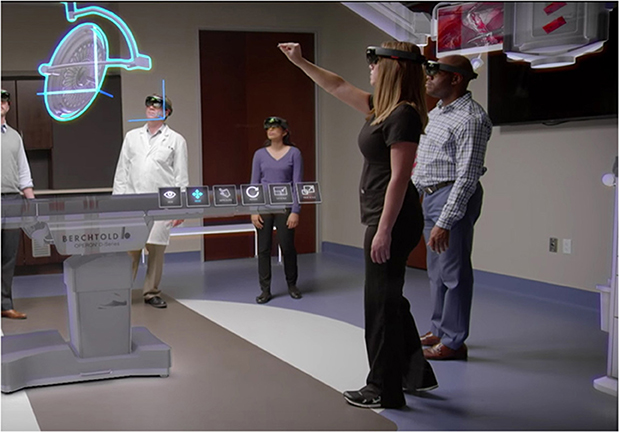
\includegraphics[width=0.5\textwidth]{vrexample.jpg}
    \caption{Mixed reality image \textcopyright Microsoft}
    \label{fig:my_label}
\end{figure}

VR and AR applications are
revolutionizing communication, collaboration, and entertainment in various
fields. Typical applications are introduced below.

\begin{table}[h]
    \begin{center}
        \begin{tabular}{|l|c|} \hline
            Service Name & Release (Establishment) Year \\ \hline
            VR Chat      & 2014                         \\
            vTime XR     & 2015                         \\ \hline
        \end{tabular}
        \caption{Virtual application using VR/AR}
    \end{center}
\end{table}

VRChat\footnote{https://hello.vrchat.com/} is a social platform centered on VR.
Users interact with other users
through avatars within a 3D environment. This platform is intended for
interaction, communication and entertainment between users and is often used
for social games, virtual events, virtual meetings, etc.

vTime XR\footnote{https://vtime.net/} is one of the social VR applications.
Users can create their own
avatars and interact with friends, family, and new people in virtual space.
This provides a real-time social experience and enhances connections with
people in remote locations.

\begin{figure}[H]
    \centering
    
\includegraphics[width=0.8\textwidth]{vtimexr.png}
    \caption{Screenshot of vTime XR \textcopyright vTime XR}
    \label{fig:my_label}
\end{figure}

\section{Pandemic}
The pandemic has fundamentally changed the way we look at virtualized services.
This crisis has had a major impact on the way businesses and individuals around
the world conduct their daily operations, prompting rapid changes in
digitalization and virtualization. One of the most notable effects of the
pandemic has been the rapid transition of many organizations to remote work.
This change has increased the demand for virtualization services such as video
conferencing, cloud storage, and online collaboration tools. Companies quickly
adopted and began operating these tools to help employees work effectively from
home.

\subsection{Expanding virtualization services}
The pandemic has significantly accelerated the adoption of virtualized
services. This change is not a temporary change; it has prompted many companies
and individuals to adopt new ways of working and communicating. As a result,
the pandemic has created new business opportunities. Demand for services and
products related to digitalization and virtualization is increasing, opening up
new markets. These services have become an important way for employees to
communicate and collaborate effectively, even remotely. These services have
seen a dramatic increase in users during the pandemic.

This article \cite{zoom_status} describes
the increase in the number of Zoom users. Before the start of the pandemic, the
number of daily meeting participants was 10 million as of December 2019. At the
start of the pandemic, in June 2020, the number of daily meeting participants
reached 300 million.

\begin{figure}[H]
    \centering
    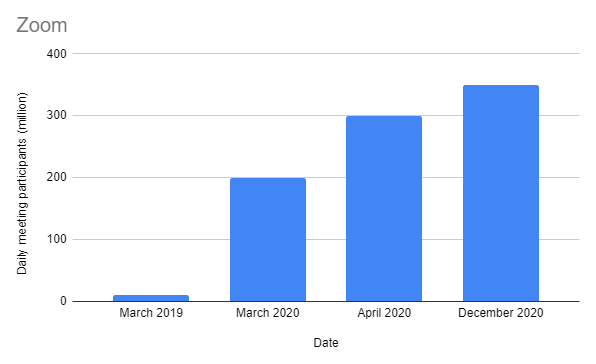
\includegraphics[width=0.6\textwidth]{zoom.png}
    \caption{Number of Zoom meeting participants}
    \label{fig:my_label}
\end{figure}

In this article \cite{teams_status},
Microsoft
Teams had 20 million users in November 2019, but 44 million users in March
2020. The number of meeting minutes per day has increased to 2.7 billion. In
April, the number rose to 75 million. It recorded a growth of
894\% from March to June 2020. In 2022, the number of users will reach 270
million.

\begin{figure}[H]
    \centering
    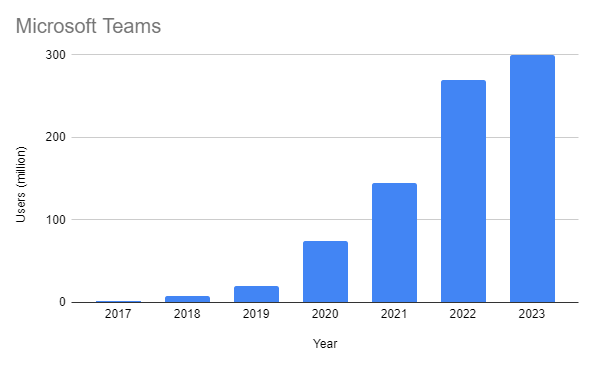
\includegraphics[width=0.6\textwidth]{teams.png}
    \caption{Number of Microsoft Teams users}
    \label{fig:my_label}
\end{figure}

This article \cite{slack_status} shows that
the number of Slack users is increasing year by year, from 2 million in 2015 to
12 million in 2019, and in 2020. reached 18 million people. The increase in the
number of users was particularly noticeable from 2019 to 2020, with an increase
of 6 million people during this period. This trend shows the growing importance
of digital communication tools, especially as the pandemic necessitated remote
working.

\begin{figure}[H]
    \centering
    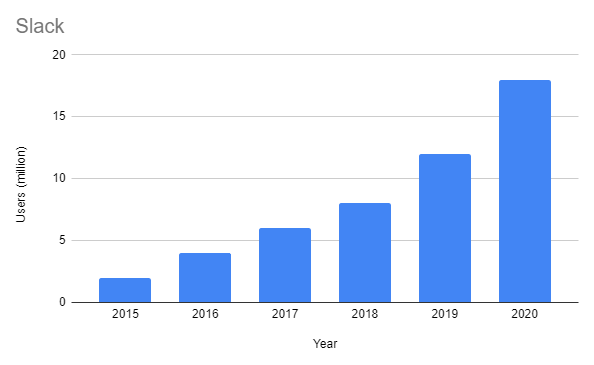
\includegraphics[width=0.6\textwidth]{slack.png}
    \caption{Number of Slack users}
    \label{fig:my_label}
\end{figure}

In this article \cite{discord_status}, the
number of Discord users will increase from 10 million in 2017 to 56 million in
2019 to 100 million in 2020. people, increasing to 175 million in 2022. This
number shows the rapid adoption and growth of the communication services
provided by Discord.

\begin{figure}[H]
    \centering
    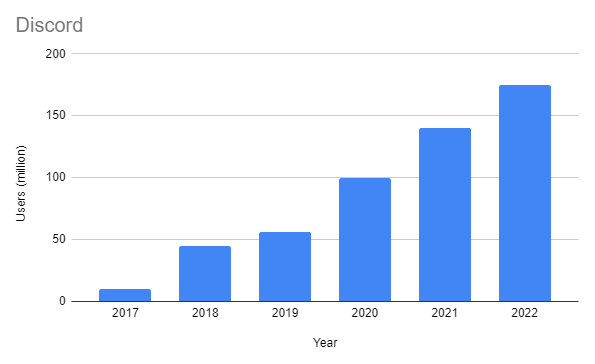
\includegraphics[width=0.6\textwidth]{discord.png}
    \caption{Number of Discord users}
    \label{fig:my_label}
\end{figure}

These data show that the pandemic has accelerated the spread of remote work and
digital communication tools, prompting many companies and individuals to adopt
new ways of working and communicating. Moreover, this change is not temporary;
it has created new business opportunities and increased demand for services and
products related to digitalization and virtualization. These services are
widely used as an important way to communicate and collaborate effectively even
from remote locations.

\subsection{Impact of virtualization services}
During the pandemic, many companies adopted (or were forced to) fully remote or
hybrid work models, leading to significant changes in the way we work and
communicate. Although this new way of working has contributed to some
improvements in employee productivity, research shows that it is actually
causing a decline in productivity. At the same time, much research has been
conducted on the blurring of boundaries between work and private life,
challenges in virtual communication, etc.

In this paper \cite{10.1371/journal.pone.0249127}, a survey of 704 academic
researchers revealed that
during the pandemic lockdown,
It talks about the loss of efficiency that comes with remote work. 94\% of
researchers surveyed indicated that they worked from home more during lockdown
than before. Of these researchers, 47\% feel that their overall research
efficiency has decreased due to increased work from home. 23\% said they felt
more efficient and 30\% said they saw no difference compared to pre-lockdown.
We are also investigating the impact of lockdown on the efficiency of people
living with children. Here, 58\% of people answered that research efficiency
has decreased overall due to increased work from home. 20\% of people felt that
their research efficiency had improved due to increased work from home. It was
found that 22\% of people felt there was no difference compared to before the
lockdown. Among researchers living with children, 71\% of 21 single parents and
57\% of 269 partnered parents said they were less productive working from home
than before the lockdown. It is written that I feel that there is.

In this paper \cite{10.1371/journal.pone.0274728}, 79\% of papers published
before the pandemic found
that working from home
increased productivity and performance. We have demonstrated that we have
improved. Meanwhile, of the papers published during the pandemic, 23\% showed a
positive effect, 38\% showed mixed results, and the remaining 38\% showed a
negative effect. The findings suggest that non-mandatory telecommuting can have
a positive impact on productivity and performance. On the other hand, if
working from home becomes compulsory and becomes full-time, or if external
factors (pandemic) come into play, the overall impact will not be as positive,
pointing out the possibility of a negative impact on productivity and
performance. Masu.

This paper \cite{Yang2022} analyzes the
impact of remote work on collaboration in a study of Microsoft employees. .
Here, we use data on emails, calendars, instant messages, video/voice calls,
and weekly work hours for 61,182 U.S. Microsoft employees in the first half of
2020 to show how company-wide remote work can improve collaboration and
communication. We are estimating the causal relationship. It shows that
company-wide remote work has made employee collaboration more static and siled,
with fewer bridges between different departments. They point out that it can be
difficult for employees to obtain and share new information on the network.

This paper \cite{inproceedings} considers different forms of remote work (e.g.
telework, remote work, virtual
work) and their impact. In particular, the pandemic has led many companies to
adopt fully remote working, which has revealed benefits such as flexibility,
cost savings, and worker autonomy.

This paper \cite{SJ2023} investigates
how remote work impacts employee productivity and happiness. We compare the
pre- and post-pandemic periods and analyze the impact of remote work on
employee productivity and well-being. The findings suggest that remote work has
had a significant impact on worker productivity and well-being both before and
after COVID-19. Although there are many benefits to working remotely, including
improved work-life balance and job satisfaction, it also points out that it can
also have negative effects, such as increased stress, anxiety, and feelings of
loneliness.

These papers explore the impact of remote work and hybrid work models on the
way we work. Research shows that while remote work can offer benefits such as
flexibility, cost savings, and worker autonomy, it can also have negative side
effects, such as reduced productivity, blurred lines between work and personal
life, and collaboration issues. It is possible that you are inviting. These
studies highlight that forced remote work has shown complex effects on
companies and employees.

\section{Predictions for virtualization services after the pandemic}
Virtualized services are expected to continue to play an
important role even after the pandemic. It will become common for many
companies to adopt flexible working arrangements and offer employees the option
of working remotely. Additionally, as technology evolves, virtualization
services have the potential to provide more advanced and efficient
functionality, enabling a more realistic communication experience.

\subsection{Post-pandemic working environment}
Enterprise use of virtualization services will continue to evolve
post-pandemic. New tools and strategies will be adopted to improve employee
productivity and satisfaction. Examples include approaches that focus on
improving virtual office environments and more efficient resource management.
In addition, through virtualization services, companies will be able to
proactively recruit and collaborate with global talent beyond geographical
constraints.

This study \cite{americans_embracing} is presented on the prevalence of work
and its
impact on American
workers. According to a survey conducted in spring 2022, 58\% of American
workers have the opportunity to work from home at least one day a week, and
35\% have the option to work from home five days a week. Remote work
opportunities span a variety of occupations and geographies, and it has become
clear that many workers prefer to work from home. This change reflects a
fundamental shift in where, when, and how work gets done.

This study \cite{covid_reshaping} shows U.S. workers Approximately 60\% can
work
from home, and of these, 83\% were
working from home before the Omicron variant spread. Many workers are now
working from home by choice, due to decreased concerns about the coronavirus
and a preference for working from home, as well as relocation from their
workplace. Although working from home has improved the balance between work and
personal life, many people feel that their connections with colleagues have
weakened. 60\% of workers say they would like to work from home even after the
spread of the coronavirus subsides. However, many workers who do not have jobs
that can be done from home, whose jobs involve direct interaction with others
at work, remain concerned about contracting the coronavirus. The frequency of
telework varies by educational background and income, and is more prevalent
among college graduates and higher income groups.

From 2020 to the present, the trend of US workers working from home has changed
significantly. Previously, concerns about coronavirus infection were the main
reason, but now many workers are working from home by choice, and the main
reason is their preference to work from home.

Among parents who work from home, the percentage of parents citing child care
as the main reason decreased from 45\% in 2020 to 32\% in 2022. At the same
time, the main reasons for workers not working from home are workplace work
productivity and personal preference, compared to lack of effective work space
or resources, opportunities for advancement, or peer pressure. This is
considered to be the reason for the lack of interest.

While many new remote workers find it easier to balance work and personal life
by working from home, many also feel less connected to their co-workers. Women
are almost twice as likely as men to say that working from home has made it
easier to advance in the workforce. Overall, new teleworkers believe that
working from home will not have a significant impact on their ability to
advance in their jobs.

This study \cite{future_of_work} found that remote work This has increased
dramatically,
with approximately
20-25\% of the workforce in developed countries now able to work from home 3-5
days a week. This is a four to five times increase compared to pre-pandemic
levels, and could result in individuals and businesses moving from large cities
to suburbs and small cities. However, it has been shown that negotiations,
important business decisions, and brainstorming sessions are best conducted in
person.

The widespread use of video conferencing during the pandemic and the newfound
acceptance of virtual meetings and other forms of remote work may also impact
business travel. It is expected to have a significant impact on airlines,
airports, hospitality industries, and food services.

We have also seen rapid growth in e-commerce and other online activities, with
many consumers discovering the convenience of digital channels. Almost
three-quarters of people who used digital channels for the first time during
the pandemic say they will continue using them even when things return to
"normal." This is driving growth in shipping, transportation, and warehousing
jobs.

In physically proximate work areas, the adoption of automation and AI is likely
to accelerate, and the proportion of work that primarily involves routine tasks
is expected to be reduced. Many companies are ramping up their investments in
automation and AI, with adoption expected to accelerate the most, especially in
work areas with high levels of human interaction.

This study \cite{what_executives_say} It shows the changes that have brought to
the working
environment and the
prospects for future hybrid work models. Organizations that have increased
productivity during the pandemic have strengthened remote leadership by
supporting and encouraging small moments of engagement among employees. Hybrid
working styles will become more common in the future, with employees expected
to be in the office one to four days a week. However, many organizations say
they still don't have a detailed vision for hybrid work and lack coordination
from top management. While most organizations saw increased individual and team
productivity and increased customer satisfaction during the pandemic, not all
organizations experienced the same improvements.

While many executives report increased employee productivity, customer
satisfaction, and engagement, it's important to focus on small connections and
training managers. In addition, implementing a hybrid model requires
redesigning processes, reviewing recruitment processes, and reconsidering the
allocation of human resources. Productivity leaders are likely to continually
iterate and fine-tune their processes as conditions change, with leading
companies completely overhauling their hiring processes and rethinking talent
allocation. As such, organizations need to evolve their management styles and
business processes to adapt to hybrid work models.

In this paper \cite{10.1371/journal.pone.0249127}, a survey of 704 academic
researchers found that
When asked about how the increase
would impact research efficiency, 29\% of those who were not yet working from
home full-time after lockdown said working from home generally improves
research output. I assumed it was a possibility. 29\% say they will be less
efficient, while 41\% think they are no different than before lockdown.
Comparing working from home and working in an office, they find that in the
office they are better at sharing ideas with colleagues, communicating with
their team, and collecting data, whereas at home they are better at working on
manuscripts and reviewing literature. Demonstrated that you are good at reading
and analyzing data.

These findings make it clear that remote and hybrid work models will continue
to play an important role in corporate environments post-pandemic. This will
require companies to adopt innovative approaches to increase flexibility in
working environments and improve employee productivity and satisfaction.
Companies can also capture new market opportunities by recruiting and
collaborating globally across geographic boundaries. As such, virtualized
services and flexible labor models will continue to be essential elements for
the growth and evolution of society and businesses.

\subsection{Adapting to virtualization}
Since the coronavirus pandemic, advanced communication technologies have been
developed to solve challenges in remote environments. New services are being
developed to encourage more flexible remote communication. For example, the
telepresence robot \cite{telepresence_robot}
enables more realistic communication by remotely controlling the robot terminal
and conducting video chats. Many telepresence robots are installed on movable
trolleys. This allows a remote operator to move from one location to another
through the robot.

Additionally, with the spread of remote services, services that support online
communication are gaining recognition. Shiseido's "TeleBeauty"
\cite{telebeauty} is
an AR filter that can
be used with online conferencing tools and video platforms. This uses a camera
app called "SnapChat" that recognizes faces and allows you to enjoy various AR
effects.

\subsection{New virtualization services using VR and AR}
Demand for new virtualization services using VR and AR applications is
increasing. The pandemic in particular has
created new services for businesses. Introducing services that bring smooth
professional communication in virtual reality and mixed reality environments.

\begin{table}[h]
    \begin{center}
        \begin{tabular}{|l|c|} \hline
            Service Name   & Release (Announcement) Year \\ \hline
            Spatial        & 2020                        \\
            Microsoft Mesh & 2021                        \\ \hline
        \end{tabular}
        \caption{Post pandemic virtual application using VR/AR}
    \end{center}
\end{table}

Spatial\footnote{https://www.spatial.io/} is a VR application designed to allow
users to collaborate within a
virtual space. The app allows users to interact through avatars and share
projects and ideas within a shared virtual environment. With features such as
real-time collaboration, 3D modeling, and data visualization, it is used in a
variety of scenarios such as education, design, and business meetings. This
article \cite{spatial_example} is using Spatial to hold an online exhibition.
is shown.
A variety of content
such as seminars, workshops, and live music will be held within the Spatial
space, allowing you to experience virtualization technology.

\begin{figure}[H]
    \centering
    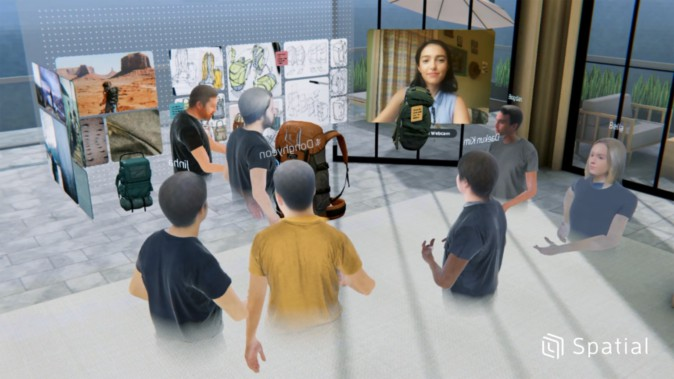
\includegraphics[width=1\textwidth]{spatial.jpg}
    \caption{Screenshot of Spatial \textcopyright Spatial}
    \label{fig:my_label}
\end{figure}

Microsoft Mesh\footnote{https://learn.microsoft.com/ja-jp/mesh/overview} is a
new platform for hybrid work and collaboration. Mesh
enables shared virtual experiences and allows users to interact across
geographic constraints. This platform is especially suitable for business
meetings, collaboration, and educational uses.

\begin{figure}[H]
    \centering
    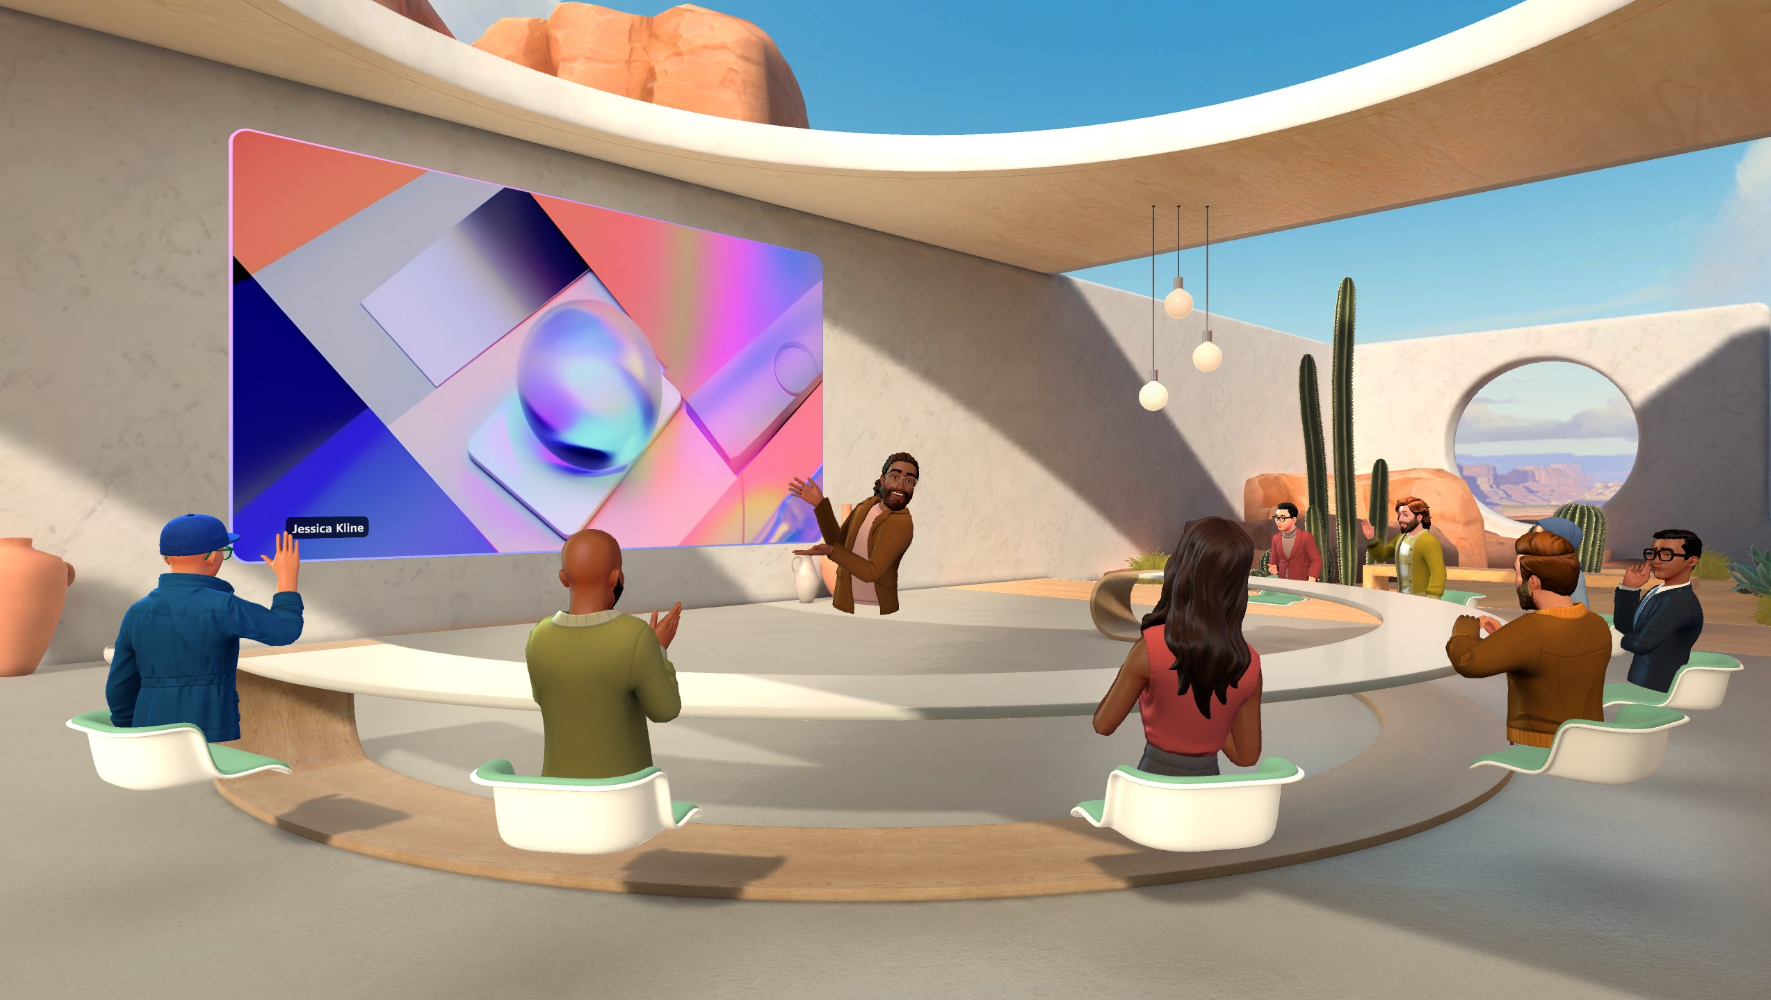
\includegraphics[width=1\textwidth]{mesh.png}
    \caption{Screenshot of Microsoft Mesh \textcopyright Microsoft Mesh}
    \label{fig:my_label}
\end{figure}

Existing VR/AR devices are increasingly being used in conjunction with existing
communication tools such as Zoom and Microsoft Teams. This makes virtual
meetings and remote collaboration a richer, more immersive experience. As VR
technology evolves, these applications continue to redefine the way people
interact in virtual spaces. What differentiates it from the aforementioned VR
Chat and vTime XR is that it brings smooth professional communication in
virtual reality and mixed reality environments.

Advances in technology are thus playing an important role in improving the
quality of communication in remote environments. New devices and applications
are improving the remote work experience and promoting more natural and
effective communication. These technological advances mean that people can more
easily connect even from remote locations, and are an important factor in
improving the quality of communication in remote environments.

\section{Conclusion}
\subsection{Benefits from the spread of remote communication}
Remote communication tools enable rapid information exchange regardless of
time and location. This speeds up decisions and keeps projects moving smoothly.
Correspondingly, companies can save money by reducing the need for physical
meeting space and business travel. Remote communication also saves
transportation costs and time. Employees can now work from home or any location
of their choice, making it easier to balance their personal and work lives.
Educational and job opportunities are also provided to people with physical
limitations and those living in remote areas. This increases the inclusiveness
of society as a whole.

\subsection{Changes from pre-pandemic to post-pandemic}
Before the pandemic, remote work and virtualization services already existed,
but were mostly used in a few niche sectors and among tech enthusiasts. Once
the pandemic began, these services quickly became a core part of daily life.
Businesses and educational institutions quickly adopted new workflows that
revolve around remote communication. Now, in the post-pandemic situation, these
services have become essential for both business and daily life.

\subsection{New virtualization service}
Virtualization services that utilize new technologies such as AR and VR provide
users with a sense of immersion. Remote communication using these technologies
provides a higher degree of collaboration and an immersive communication
experience. However, due to the high cost of these technologies, not all users
or businesses can easily adopt them. Additionally, with the spread of
virtualization services, services such as telepresence robots are also becoming
more popular. Such services will need to continue to be developed to improve
remote communication.

\subsection{Spread of full remote work/hybrid work}
Fully remote work gives employees the freedom to work from anywhere. This can
reduce commuting time, improve work-life balance, and increase personal
productivity. Hybrid work, or a combination of remote and office work, has
become widespread in the wake of the pandemic. This workstyle is attracting
attention as a new way of working that meets the needs of employees while
balancing flexibility and productivity.

\subsection{Strengthening international communication}
Virtualization services have reduced the barriers to international
communication. Language barriers are gradually being overcome due to advances
in technology. This fosters collaboration between different cultures and
academic disciplines. You will be able to hire talented people regardless of
geographic constraints. This allows us to build diverse teams and work with a
global perspective. On the other hand, when users from different countries use
remote services, for example, there are issues that cannot be addressed by
technology, such as time differences. Virtualization services are by no means a
panacea.

\subsection{Future work and risk responses}
The proliferation of remote work and virtualized services has brought new
challenges to the fore, including weakened relationships, security issues,
technological hurdles, and a blurring of the line between work and personal
life. To address these issues, it is important to educate users, take
appropriate security measures, and emphasize work-life balance. The pandemic
has revealed the importance of virtualized services and has had a huge impact
on the way we work and communicate in the future. The lessons learned from this
experience will be useful for future technological development and the
evolution of society.

\bibliographystyle{plain}
\bibliography{references.bib}

\end{document}
